\documentclass[a4paper, 11pt]{article}

\usepackage{amsfonts,amssymb}
\usepackage{amsmath}
\parindent 0px
\usepackage{float}
\usepackage{enumerate}    
\usepackage[hidelinks]{hyperref}     
\usepackage[a4paper,margin=1in,footskip=0.25in]{geometry}  
\usepackage{graphicx}
\usepackage{attachfile}
\usepackage{bbm}
\usepackage{color}
\usepackage{colortbl}
\usepackage{multicol}
\usepackage{multirow}
\usepackage{natbib}
\usepackage[tablegrid]{vhistory}
\usepackage{ulem}
\usepackage{verbatim}
\usepackage{xspace}
\usepackage[ruled, vlined]{algorithm2e}
\usepackage{booktabs}
\usepackage{placeins}
\usepackage{seqsplit}
\usepackage{caption}
\usepackage{xcolor}
\usepackage{float}

\title{Pairs Trading Strategy Design and Backtest}
\author{Prasoon Gupta}
%\date{}

\begin{document}

\maketitle

\pagebreak

\tableofcontents

\pagebreak

\section{Introduction}
Cointegration is known as a model for a long-term relationship, which is a short-cut taken for the ease of explanation. It is illustrative to contrast cointegration and correlation, while, in fact, multiple scenarios are possible: correlated series can run away from each other, while cointegrated series might be seemingly unrelated. Correlation suffers from shortcomings of its measurement: it reflects co-movement on the small time-scale only and, when measured over the long term, compounds to abnormally high values. Correlation among equities is usually range-bound, so it is a fundamentally uncertain parameter. Cointegration too have an element of uncertainty: the spread produced by cointegrated time series is stationary and mean-reverting around some
linear equilibrium level. The tie-in among cointegrated series is not exact.

Economic theory suggests that many time series datasets will move together, fluctuating around a long-run equilibrium. In econometrics and statistics, this long-run equilibrium is tested and measured using the concept of cointegration.\\
Cointegration occurs when two or more nonstationary time series:

\begin{itemize}
\item Have a long-run equilibrium.
\item Move together in such a way that their linear combination results in a stationary time series.
\item Share an underlying common stochastic trend.
\end{itemize}

To understand the mathematics of cointegration, let's consider a group of time series, which is composed of three separate time series

$$y_1 = (y_{11}, y_{12}, \ldots, y_{1t})$$
$$y_2 = (y_{21}, y_{22}, \ldots, y_{2t})$$
$$y_3 = (y_{31}, y_{32}, \ldots, y_{3t})$$

All three series are nonstationary time series.
Cointegration implies that while $y_1$,$y_2$ and $y_3$ are independently nonstationary, they can be combined in a way that their linear combination is stationary :

$$\beta_{coint} Y_t = \beta_1 y_{1t} + \beta_2 y_{2t} + \beta_3 y_{3t} \sim I(0)$$

\textbf{The Cointegrating Vector} In the context of cointegration $\beta_{coint} $ is commonly known as the cointegrating vector. This vector:

\begin{itemize}
\item Dictates how cointegrating series are combined.
\item Does not have to be unique - there can be multiple ways of cointegrating.
\end{itemize}

Normalization Because there can be multiple cointegrating vectors that fit the same economic model, we must impose identification restrictions to normalize the cointegrating vector for estimation.

A common normalization of the cointegrating vector is to set $\beta_{coint} = ( 1,  -\beta_2, \ldots, -\beta_N)$
For example, applying these restrictions to our earlier system yields

$$\beta_{coint} Y_t = y_{1t} - \beta_2 y_{2t} - \beta_3 y_{3t} \sim I(0)$$

Part of the appeal of this normalization is that it can be rewritten in a standard regression form

$$ e_t = y_{1t} - \beta_2 y_{2t} - \beta_3 y_{3t}$$

$$ e_t = \beta_{coint} Y_t $$
where $e_t$is a stationary cointegrating error component which is also called spread.\\

The spread is a stationary and autoregressive process, which gives it the mean reversion property. But it is not an integrated process, \textbf{integrated of order zero}. In comparison, a non-stationary $y_{i,t}$ is \textbf{integrated} because it can be decomposed into the infinite sum of residuals that are econometric moving averages.Building models of non-stationary time series by means of a regression. We will see below how regression for $y_t$ is a static model - requires a genuine long-run relationship among the series. \textbf{In the absence of a long-run run relationship, there is no way to tie the non-stationary variables to produce a stationary spread}. A spurious regression will show the high goodness of fit $R^2$ but it has been proven that its coefficients are random variables that do not converge to their true value of zero. Therefore, the common statistical inference fails in the special case of spurious regression. However, it is not possible to detect that without building a further model for cointegration.

\pagebreak

\section{Exploratory analysis to identify Cointegrated pairs}

Our first step is to decide the stock universe and identify the cointegrated pairs . It is very important that this is based on economic relationships such as companies with similar businesses, else it might be spurious. We have taken  constituents of \textbf{US Financial Sector} which are categorized as \textbf{Financial Services} companies. We take the daily closing price for these 15 stocks for from period Jan-20 to Jun-22.

\begin{figure}[ht]
	\centering
	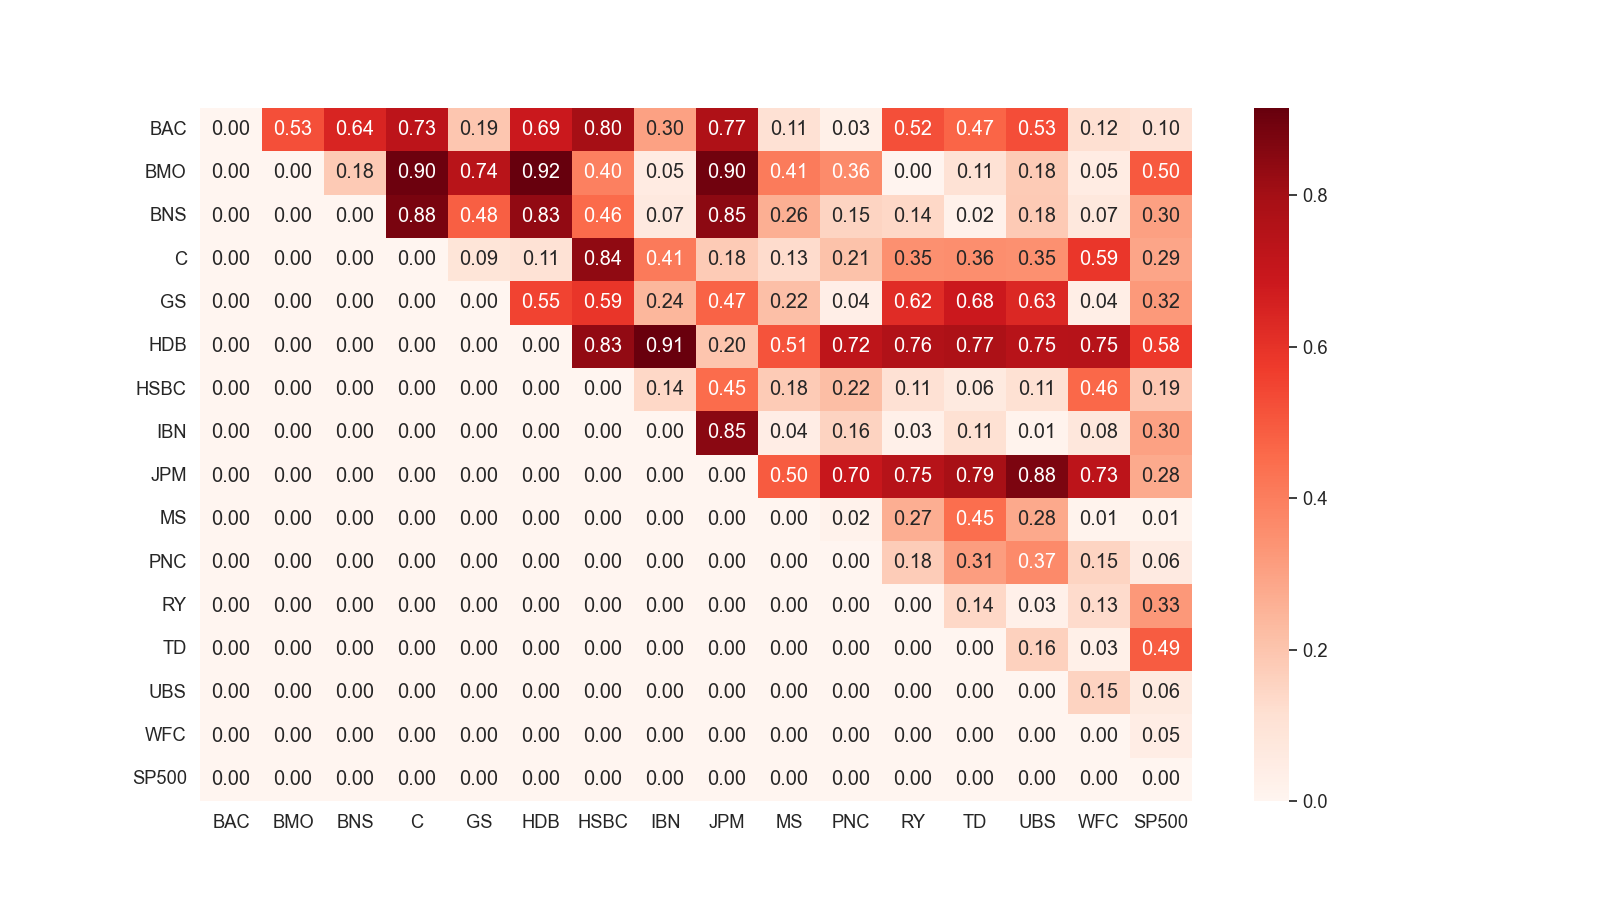
\includegraphics[width = 1.2\textwidth]{Figures/pair_identify.png}
	\caption{Equity Pair Cointegration Score}
	\label{fig:eq_cointegration_score}
\end{figure}
\FloatBarrier	

Based on results of Fig \ref{fig:eq_cointegration_score}, we select stocks \textbf{BAC(Bank of Americal Corp) and PNC(The PNC Financial Services) as a potential candidate} for cointegration analysis since p -value from cointegraton test is small and less than 0.05 threshold.

\pagebreak

\section{Cointegration Analysis and Mean Reversion process}

\subsection{Stock Prices data}

We split prices data for BAC and PNC into training and test sets along with S\&P 500 index which will be used as a benchmark index for returns comparison \& analysis. This is to ensure that our decision to select a cointegrated pair is based on the training dataset and backtesting is done using out of sample test dataset.\\

Time series data are sequential in nature and are characterised by the correlation between observations. Classical cross-validation techniques such as KFold assume the samples are independent and identically distributed, and would result in poor estimates when applied on time series data.\\

To preserve the order and have training set occur prior to the test set, we split prices data in 80:20 ratio i.e. 80 for training set and 20 for test set sequentially. And therefore training set contains data for 2 years period(Jan-20 to Dec-21) and similarly, test set contains data for 6 months(Jan-22 to Jun-22).\\

\begin{figure}[ht]
	\centering
	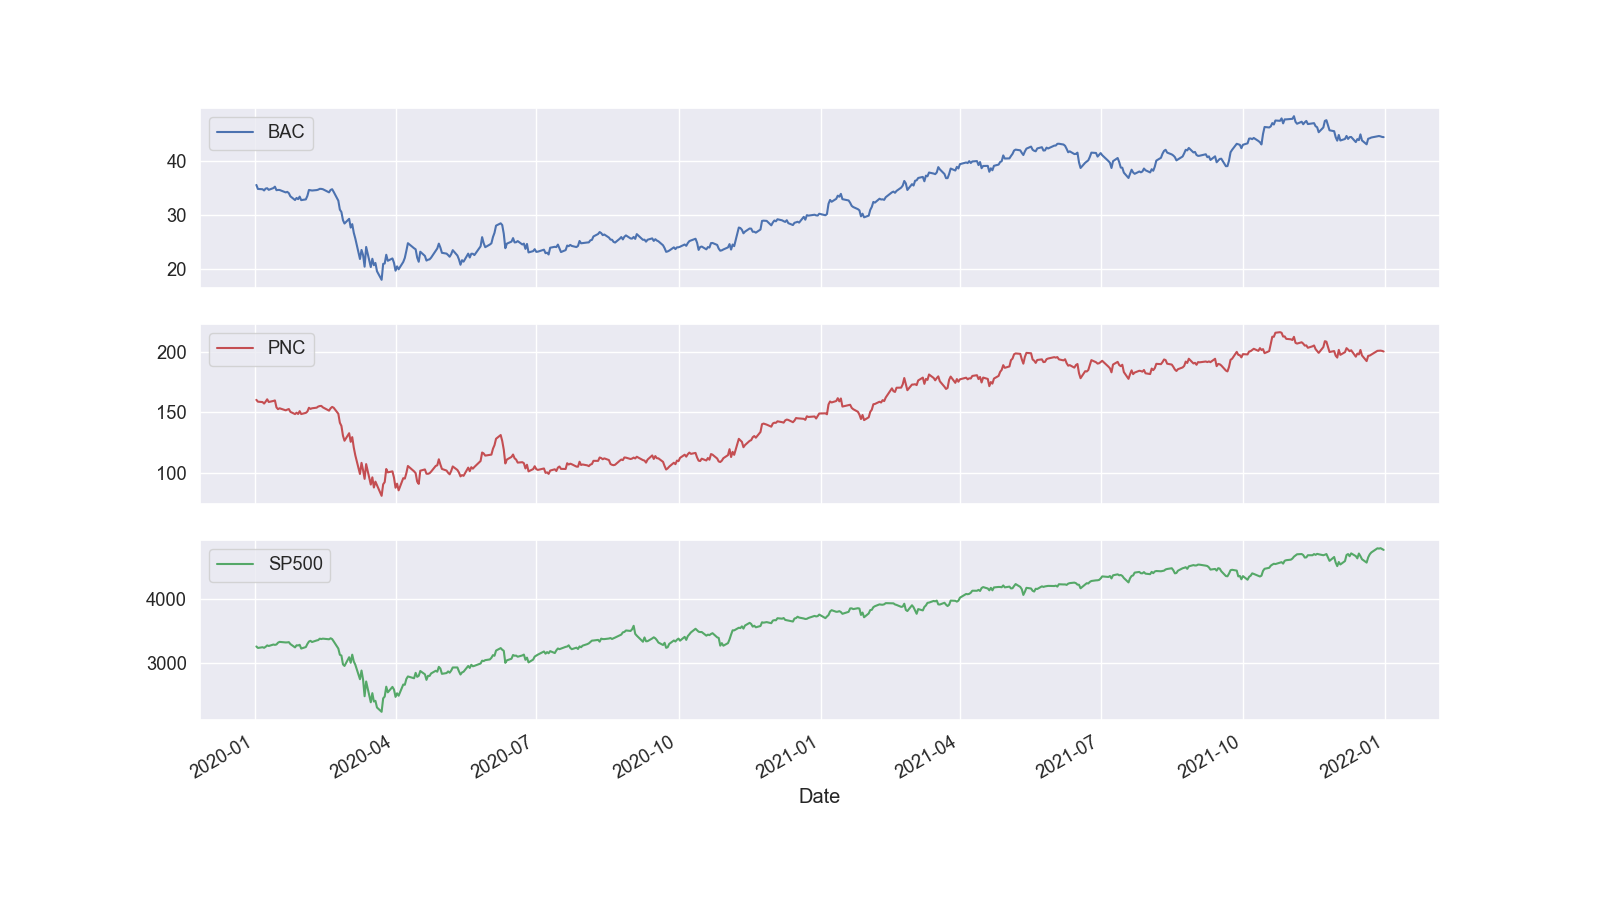
\includegraphics[width = 1\textwidth]{Figures/stock_prices.png}
	\caption{Stock Prices Movement}
	\label{fig:stock_prices}
\end{figure}
\FloatBarrier	

\begin{figure}[ht]
	\centering
	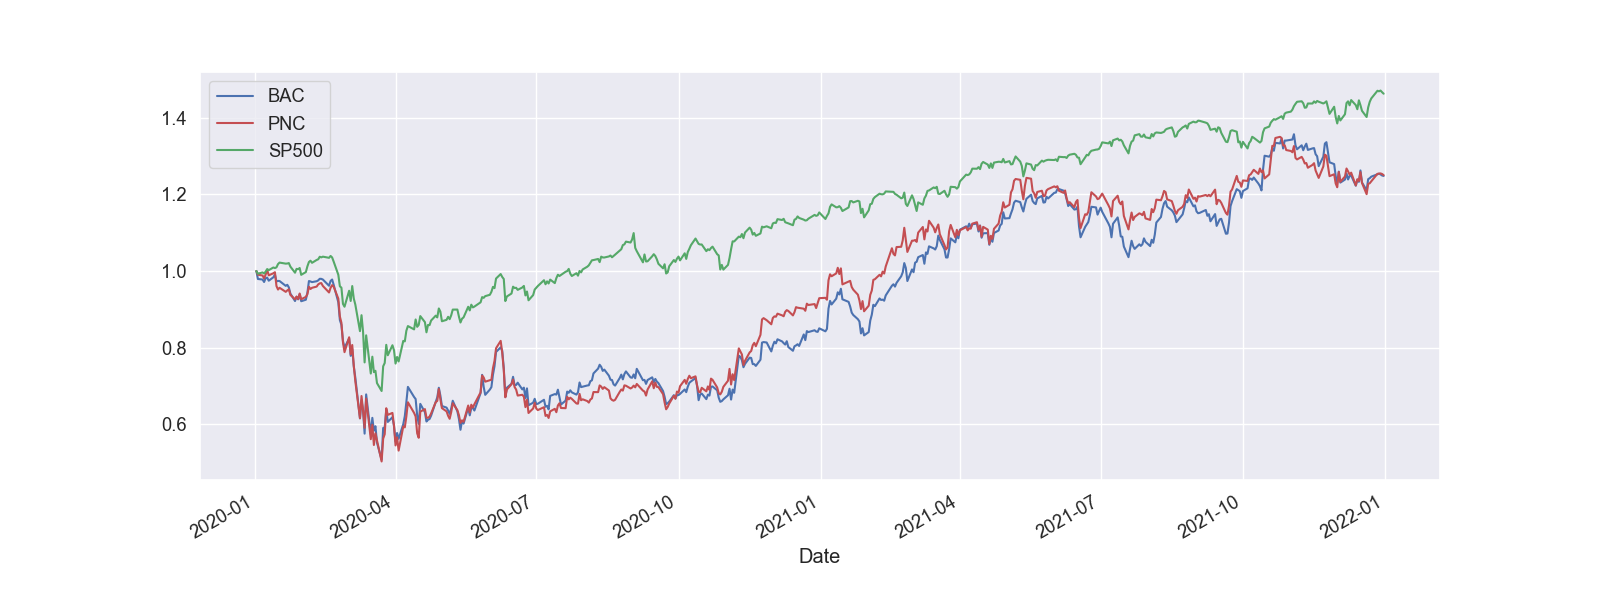
\includegraphics[width = 1\textwidth]{Figures/stock_prices_norm.png}
	\caption{Normalized Stock Prices Movement}
	\label{fig:stock_prices_norm}
\end{figure}
\FloatBarrier

Above are the price charts of BAC, PNC and S\&P 500 for training set both in actual and normalized terms i.e. make day 1 prices as unit prices. On Cursory look at these charts, we can say that BAC and PNC prices move together and seem cointegrated. However, we need to perform statistical tests to confirm this hypothesis.
Cointegration testing is sensitive to the initial value(normalising to start at one), also this allows comparison of P\&L easily.

\pagebreak

\subsection{Stationarity check of daily returns}

We plot log returns of BAC, PNC and S\&P 500 and it seems all three return time series are stationary. However, we will perform Augmented Dickey Fuller(ADF) test to confirm the same.\\

\begin{figure}[ht]
	\centering
	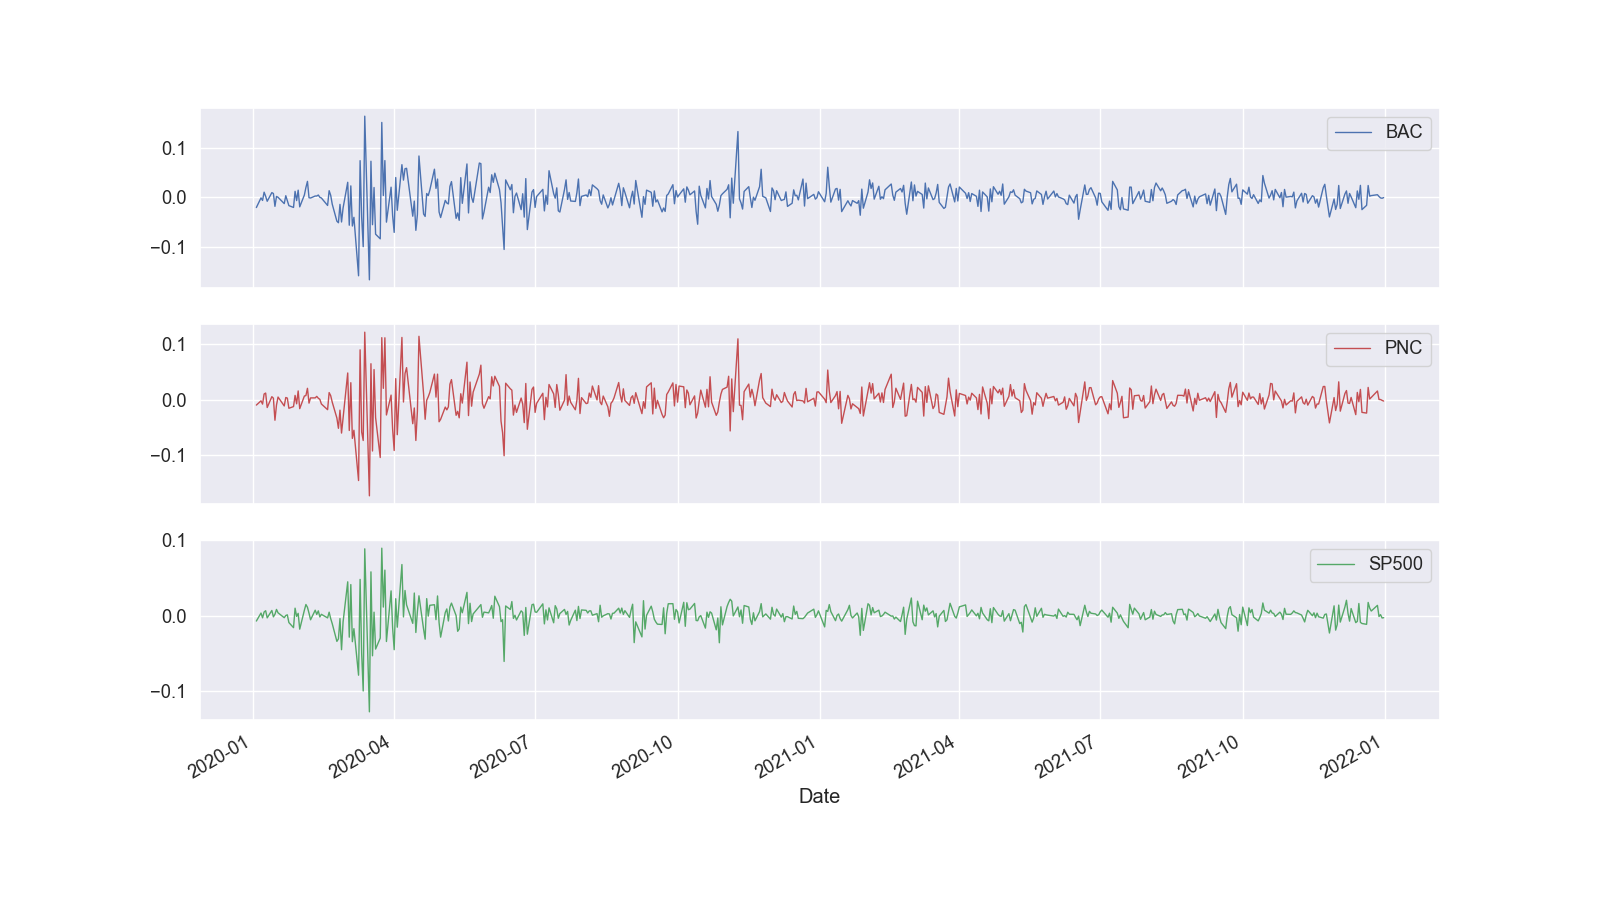
\includegraphics[width = 1\textwidth]{Figures/returns.png}
	\caption{Stock Log Returns}
	\label{fig:retuns}
\end{figure}
\FloatBarrier

\textbf{Augmented Dickey Fuller(ADF) test:}\\

Dickey Fuller test is a statistical test that is used to check for stationarity in time series. This is a type of unit root test, through which we find if the time series is having any unit root. Unit root is a feature of time series that indicates if there is any stochastic trend in the time series that drives it away from its mean value. Presence of unit root makes a time series non-stationary and as a result it leads to difficulties in deriving statistical inferences from the time series and future predictions.

Dickey Fuller test assumes a AR(1) type time series model and it is represented mathematically as the Dickey-Fuller test is testing if  $\phi = 0$

$$ y_t = \alpha + \beta t + \phi y_{t-1} + e_t $$

this can be written as :
$$\Delta y_t = y_t-y_{t-1}= \alpha + \beta t + \gamma y_{t-1} + e_t $$ 

where $\gamma = \phi -1 $ 

The Augmented Dickey-Fuller test allows for higher-order autoregressive processes by including  $\Delta y_{t-p}$ in the model. But our test is still if $\gamma =0 $
 
$$\Delta y_t = \alpha + \beta t + \gamma y_{t-1} + \delta_1 \Delta y_{t-1} + \delta_2 \Delta y_{t-2} + \dots $$

\textbf{we drop constant drift term and time dependent trend term since these modifications can create temporary
dependency and give over-fitted results}. Additionally, we restrict number of lags to 1. Based on aforementioned modifications, equation is as follows

$$\Delta y_t = \gamma y_{t-1} + \delta_1 \Delta y_{t-1} + e_t$$ 

\textbf{H0 (Null hypothesis)}: Time series data has unit root and is non-stationary, $\gamma = 0$ 

\textbf{H1 (Alternative hypothesis)} Time series data has no unit root and is stationary\\

We want to REJECT the null hypothesis for this test, so we want a p-value of less that 0.05 (or smaller).

\subsubsection{Stationarity check for BAC stock log-returns time series - I(0) process}

\begin{table}[!ht] 
\centering 
\resizebox{0.7\textwidth}{!} { 
\begin{tabular}{rrrr}
\toprule
test statistics & p-value & No of lagged values & No of observations \\
\midrule
-5.9331 & 0.0000 & 9 & 494 \\
\bottomrule
\end{tabular}} 
\caption {ADF test output on BAC Returns} 
\label {adf_bac} 
\end{table} 
\FloatBarrier

From Augmented Dickey-Fuller test output on BAC log-returns time series, we conclude that it is stationary since p-value is insignificant and not breaching ADF distribution threshold. And Hence, BAC log-returns is integrated process of order zero.

\subsubsection{Stationarity check for PNC stock log-returns time series - I(0) process}

\begin{table}[!ht] 
\centering 
\resizebox{0.7\textwidth}{!} { 
\begin{tabular}{rrrr}
\toprule
test statistics & p-value & No of lagged values & No of observations \\
\midrule
-6.1579 & 0.0000 & 8 & 495 \\
\bottomrule
\end{tabular}} 
\caption {ADF test output on PNC Returns} 
\label {adf_pnc} 
\end{table} 
\FloatBarrier

We perform similar Augmented Dickey-Fuller test on PNC log-returns time series and conclude that it is stationary since p-value is insignificant and not breaching ADF distribution threshold. And Hence, PNC log-returns is integrated process of order zero.

\subsubsection{Stationarity check for S\&P 500 index log-returns time series - I(0) process}

\begin{table}[!ht] 
\centering 
\resizebox{0.7\textwidth}{!} { 
\begin{tabular}{rrrr}
\toprule
test statistics & p-value & No of lagged values & No of observations \\
\midrule
-6.2267 & 0.0000 & 8 & 495 \\
\bottomrule
\end{tabular}} 
\caption {ADF test output on S\&P500 Returns} 
\label {adf_sp500} 
\end{table} 
\FloatBarrier

We perform similar Augmented Dickey-Fuller test on S\&P 500 index log-returns time series and conclude that it is stationary since p-value is insignificant and not breaching ADF distribution threshold. And Hence, S\&P 500 index log-returns is integrated process of order zero.

\pagebreak
\subsection{VAR Model fitting : Matrix form representation}

VAR(vector autoregressive) models are used for multivariate time series. The structure is that each variable is a linear function of past lags of itself and past lags of the other variables.

A VAR(1) in three variables can be written in matrix form (more compact notation) as

$$\begin{pmatrix} {y}_{1t} \\ y_{2t} \\ y_{3t}\end{pmatrix} =   
\begin{pmatrix} a_{10} \\ a_{20} \\ a_{30} \end{pmatrix} + \begin{bmatrix} a_{11} & a_{12} & a_{13} \\ a_{21} & a_{22} & a_{23} \\ a_{31} & a_{32} & a_{33}\end{bmatrix}\begin{pmatrix} y_{1t-1} \\ y_{2t-1}  \\ y_{3t-1}\end{pmatrix} + 
\begin{pmatrix} \epsilon_{1t} \\ \epsilon_{2t} \\ \epsilon_{3t}
\end{pmatrix}$$

or, more compactly,
$$ y_t = A_0 + A_1 y_{t-1} + \epsilon_t,$$

where, $$y_t = \begin{pmatrix} y_{1t} \\ y_{2t} \\ y_{3t}\end{pmatrix}, A_0 = \begin{pmatrix} a_{10} \\ a_{20} \\ a_{30} \end{pmatrix}, A_1= \begin{bmatrix} a_{11} & a_{12} & a_{13} \\ a_{21} & a_{22} & a_{23} \\ a_{31} & a_{32} & a_{33}\end{bmatrix} \text{and   } \epsilon_t = \begin{pmatrix} \epsilon_{1t} \\ \epsilon_{2t} \\\epsilon_{3t} \end{pmatrix}.$$

Basically, such a model implies that everything depends on everything. But as can be seen from this formulation, each row can be written as a separate equation, so that 
$$ y_{1t} = a_{10} + a_{11} y_{1t-1} + a_{12} y_{2t-1} + a_{13} y_{3t-1} + \epsilon_{1t} $$
$$ y_{2t} = a_{20} + a_{21} y_{1t-1} + a_{22} y_{2t-1} + a_{23} y_{3t-1} + \epsilon_{2t} $$
$$ y_{3t} = a_{30} + a_{31} y_{1t-1} + a_{32} y_{2t-1} + a_{33} y_{3t-1} + \epsilon_{3t} $$

Hence, the VAR model can be rewritten as a series of individual ADL models as described above. In fact, it is possible to estimate VAR models by estimating each equation separately.\\

For our analysis, endogenous variables in VAR(1) model are log returns of BAC, PNC and S\&P 500 stocks which are stationary in nature. And therefore, we can rewrite above equations as follows

$$ R^{BAC}_{t} = a_{10} + a_{11} R^{BAC}_{t-1} + a_{12} R^{PNC}_{t-1} + a_{13} R^{SP500}_{t-1} + \epsilon_{1t} $$

$$ R^{PNC}_{t} = a_{20} + a_{21} R^{BAC}_{t-1} + a_{22} R^{PNC}_{t-1} + a_{23} R^{SP500}_{t-1} + \epsilon_{2t} $$

$$ R^{SP500}_{t} = a_{30} + a_{31} R^{BAC}_{t-1} + a_{32} R^{PNC}_{t-1} + a_{33} R^{SP500}_{t-1} + \epsilon_{3t} $$ \\

we perform regression between stationary variables which are daily returns of of BAC, PNC and S\&P 500 stocks. To identify optimal p lags for model selection, we perform BIC test 


\begin{table}[!ht] 
\centering 
\resizebox{0.2\textwidth}{!} { 
\begin{tabular}{rr}
\toprule
Lag & BIC Value \\
\midrule
1 & -25.2083 \\
2 & -25.1611 \\
3 & -25.1131 \\
4 & -25.0404 \\
5 & -24.9349 \\
6 & -24.8668 \\
7 & -24.8440 \\
8 & -24.7799 \\
9 & -24.7239 \\
10 & -24.6415 \\
\bottomrule
\end{tabular}} 
\caption {BIC test output on VAR Model} 
\label {var_bic} 
\end{table} 
\FloatBarrier

The BIC statistic is calculated as follows 

BIC = -2 * LL + log(N) * k

Where log() has natural logarithm, LL is the log-likelihood of the model, N is the number of observations in the dataset, and k is the number of parameters in the model. The model with the lowest BIC is selected and based on output, we select optimal lag as 1.\\

To investigate whether the daily returns depend on their past values, we fit the VAR(1) model to daily returns.
The question now is whether the estimated coefficients are significantly different from zero,we inspect the p-values. We will reject the hypothesis that a regression coefficient is zero if the corresponding p-value is less than 5\%.\\

The output of VAR model conclude that past lagged values cannot be used to predict the future returns for these two equities. Nevertheless, we observe that BAC and PNC stocks returns are dependent on S\&P 500 lagged returns
\\

\textbf{Summary of VAR Model}\\

\begin{tabular}{lclc}
\toprule
%\textbf{Summary of Regression Results}         &         &    & \\\\
\textbf{Model:   VAR}         &              &    & \\
\textbf{Method:  OLS}        &              &    & \\
\end{tabular}

\begin{tabular}{lclc}
\toprule
\textbf{No of Equations:}       &  3.0000 & \textbf{  BIC:     } &    -25.2083  \\
\textbf{Nobs):} &  503.0000 & \textbf{  Jarque-Bera (HQIC):  } &    -25.2695  \\
\textbf{Log likelihood:}          & 4236.03 & \textbf{  FPE:          } &   1.01964e-11  \\
\textbf{AIC:}      &  -25.3090 & \textbf{  Cond. No.          } &     9.95701e-12  \\
\bottomrule
\\
\end{tabular}

\begin{tabular}{lcccc}
\textbf{Results for equation BAC}             & \textbf{coefficient} & \textbf{std. error} & \textbf{t-stat} & \textbf{prob} \\
\midrule
\textbf{const} &      0.000752  &        0.001242     &    0.606  &         0.545           \\
\textbf{L1.BAC}   &       -0.046394 &        0.113398      &   -0.409  &         0.682         \\
\textbf{L1.PNC}   &       0.006555  &        0.111656     &   0.059  &         0.953         \\
\textbf{L1.SP500}   &       -0.331001  &        0.121533     &   -2.724  &         0.006         \\
\bottomrule
\\
\end{tabular}

\begin{tabular}{lcccc}
\textbf{Results for equation PNC}              & \textbf{coefficient} & \textbf{std. error} & \textbf{t-stat} & \textbf{prob} \\
\midrule
\textbf{const} &      0.0.000747  &        0.001231     &    0.607  &         0.544           \\
\textbf{L1.BAC}   &      -0.009388  &        0.112455      &   -0.083  &         0.933         \\
\textbf{L1.PNC}   &        -0.030619  &        0.110727     &   -0.277  &         0.782         \\
\textbf{L1.SP500}   &       -0.349219   &        0.120522     &   -2.898  &         0.004         \\
\bottomrule
\\
\end{tabular}

\begin{tabular}{lcccc}
\textbf{Results for equation SP500}             & \textbf{coefficient} & \textbf{std. error} & \textbf{t-stat} & \textbf{prob} \\
\midrule
\textbf{const} &      0.000988  &        0.000703     &    1.406  &         0.160           \\
\textbf{L1.BAC}   &      -0.045830  &        0.064187      &  -0.714  &         0.475        \\
\textbf{L1.PNC}   &        0.009645  &        0.063201     &   0.153  &         0.879         \\
\textbf{L1.SP500}   &       -0.264782    &        0.068791     &   -3.849  &         0.000         \\
\bottomrule
\end{tabular}


\pagebreak
\subsection{Cointegration Analysis}

In this section we implement the Engle-Granger procedure to confirm (or not) if the pair is cointegrated and therefore, suitable for trade design.

\subsubsection{Engle-Granger Procedure Step 1}

\begin{enumerate}[A.]
\item
\textbf{Regression of PNC Financial Services(PNC) stock on Bank of America(BAC) stock }\\

We are now ready to perform the 1st step of the Engle-Granger procedure which is to estimate the model. Here, we do linear regression of PNC prices on BAC prices.

$$ PNC_t = \alpha + \beta * BAC_t + e_t $$
$\alpha = -0.0110, \beta = 1.0284 $ and residual is as follow 

$$ e_t = PNC_t + 0.0110 - 1.0284 * BAC_t $$

where $ \beta_{coint} = [1,-1.0284] $

\textbf{Summary of Regression - PNC prices on BAC prices} 
\begin{center}
\begin{tabular}{lclc}
\toprule
\textbf{Dep. Variable:}    &       PNC        & \textbf{  R-squared:         } &     0.977   \\
\textbf{Model:}            &       OLS        & \textbf{  Adj. R-squared:    } &     0.977   \\
\textbf{Method:}           &  Least Squares   & \textbf{  F-statistic:       } & 2.185e+04   \\
\textbf{Date:}             & Tue, 16 Jan 2024 & \textbf{  Prob (F-statistic):} &     0.00    \\
\textbf{Time:}             &     09:20:28     & \textbf{  Log-Likelihood:    } &    964.25   \\
\textbf{No. Observations:} &         505      & \textbf{  AIC:               } &    -1924.   \\
\textbf{Df Residuals:}     &         503      & \textbf{  BIC:               } &    -1916.   \\
\textbf{Df Model:}         &           1      & \textbf{                     } &             \\
\textbf{Covariance Type:}  &    nonrobust     & \textbf{                     } &             \\
\bottomrule
\end{tabular}
\begin{tabular}{lcccccc}
               & \textbf{coef} & \textbf{std err} & \textbf{t} & \textbf{P$> |$t$|$} & \textbf{[0.025} & \textbf{0.975]}  \\
\midrule
\textbf{const} &      -0.0110  &        0.007     &    -1.641  &         0.101        &       -0.024    &        0.002     \\
\textbf{BAC}   &       1.0284  &        0.007     &   147.819  &         0.000        &        1.015    &        1.042     \\
\bottomrule
\end{tabular}
\begin{tabular}{lclc}
\textbf{Omnibus:}       & 18.586 & \textbf{  Durbin-Watson:     } &    0.077  \\
\textbf{Prob(Omnibus):} &  0.000 & \textbf{  Jarque-Bera (JB):  } &   13.715  \\
\textbf{Skew:}          &  0.298 & \textbf{  Prob(JB):          } &  0.00105  \\
\textbf{Kurtosis:}      &  2.456 & \textbf{  Cond. No.          } &     8.27  \\
\bottomrule
\end{tabular}
%\caption{OLS Regression Results}
\end{center}

Notes: \newline
 [1] Standard Errors assume that the covariance matrix of the errors is correctly specified.

\begin{figure}[ht]
	\centering
	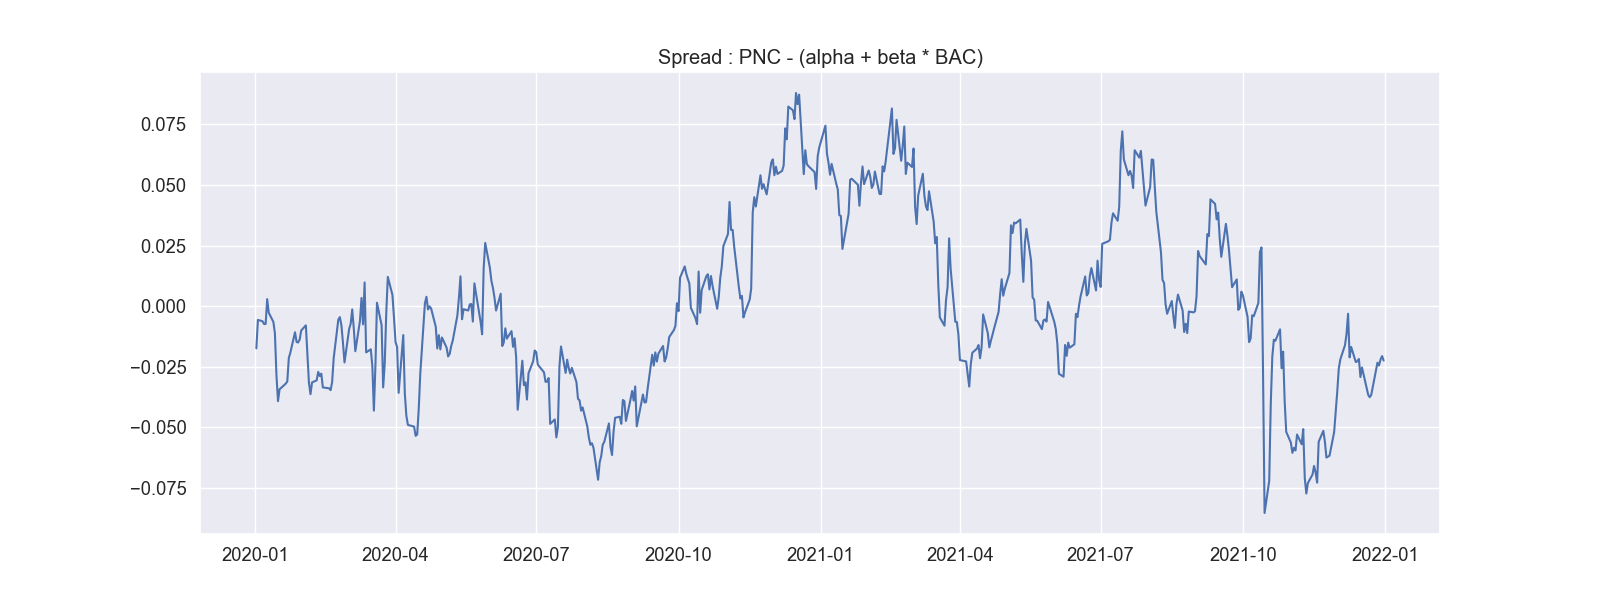
\includegraphics[width = 1\textwidth]{Figures/spread_pnc.png}
	\caption{Residual/Spread of Regression of PNC on BAC}
	\label{fig:spread_pnc}
\end{figure}
\FloatBarrier

$$\Delta e^{PNC}_t = \gamma e^{PNC}_{t-1} + \delta_1 \Delta e^{PNC}_{t-1} + \epsilon_t$$\\

The question now is whether the Cointegrated PNC residual $e^{PNC}_t$ is stationary or not. We perform Augmented Dickey-Fuller Test on this Cointegrated PNC residual with lag 1 and conclude that it is stationary since p-value is less than 0.05 threshold.

\begin{table}[!ht] 
\centering 
\resizebox{0.7\textwidth}{!} { 
\begin{tabular}{rrrr}
\toprule
test statistics & p-value & No of lagged values & No of observations \\
\midrule
-3.2236 & 0.0187 & 1 & 503 \\
\bottomrule
\end{tabular}} 
\caption {ADF test output on PNC Residual/Spread} 
\label {adf_pnc_bac} 
\end{table} 
\FloatBarrier

\item
\textbf{Regression of Bank of America(BAC) stock on PNC Financial Services(PNC) stock}\\

Here, we do linear regression of BAC prices on PNC prices.

$$ BAC_t = \alpha + \beta * PNC_t + e_t $$
$\alpha = 0.0315, \beta = 0.9505 $ and residual is as follow 

$$ e_t = BAC_t - 0.0315 - 0.9505 * PNC_t $$

where $ \beta_{coint} = [1,-0.9505] $

\textbf{Summary of Regression - BAC prices on PNC prices} 
\begin{center}
\begin{tabular}{lclc}
\toprule
\textbf{Dep. Variable:}    &       BAC        & \textbf{  R-squared:         } &     0.977   \\
\textbf{Model:}            &       OLS        & \textbf{  Adj. R-squared:    } &     0.977   \\
\textbf{Method:}           &  Least Squares   & \textbf{  F-statistic:       } & 2.185e+04   \\
\textbf{Date:}             & Wed, 17 Jan 2024 & \textbf{  Prob (F-statistic):} &     0.00    \\
\textbf{Time:}             &     09:04:54     & \textbf{  Log-Likelihood:    } &    984.15   \\
\textbf{No. Observations:} &         505      & \textbf{  AIC:               } &    -1964.   \\
\textbf{Df Residuals:}     &         503      & \textbf{  BIC:               } &    -1956.   \\
\textbf{Df Model:}         &           1      & \textbf{                     } &             \\
\textbf{Covariance Type:}  &    nonrobust     & \textbf{                     } &             \\
\bottomrule
\end{tabular}
\begin{tabular}{lcccccc}
               & \textbf{coef} & \textbf{std err} & \textbf{t} & \textbf{P$> |$t$|$} & \textbf{[0.025} & \textbf{0.975]}  \\
\midrule
\textbf{const} &       0.0315  &        0.006     &     4.996  &         0.000        &        0.019    &        0.044     \\
\textbf{PNC}   &       0.9505  &        0.006     &   147.819  &         0.000        &        0.938    &        0.963     \\
\bottomrule
\end{tabular}
\begin{tabular}{lclc}
\textbf{Omnibus:}       &  8.373 & \textbf{  Durbin-Watson:     } &    0.077  \\
\textbf{Prob(Omnibus):} &  0.015 & \textbf{  Jarque-Bera (JB):  } &    7.338  \\
\textbf{Skew:}          & -0.228 & \textbf{  Prob(JB):          } &   0.0255  \\
\textbf{Kurtosis:}      &  2.625 & \textbf{  Cond. No.          } &     8.08  \\
\bottomrule
\end{tabular}
%\caption{OLS Regression Results}
\end{center}

Notes: \newline
 [1] Standard Errors assume that the covariance matrix of the errors is correctly specified.

\begin{figure}[ht]
	\centering
	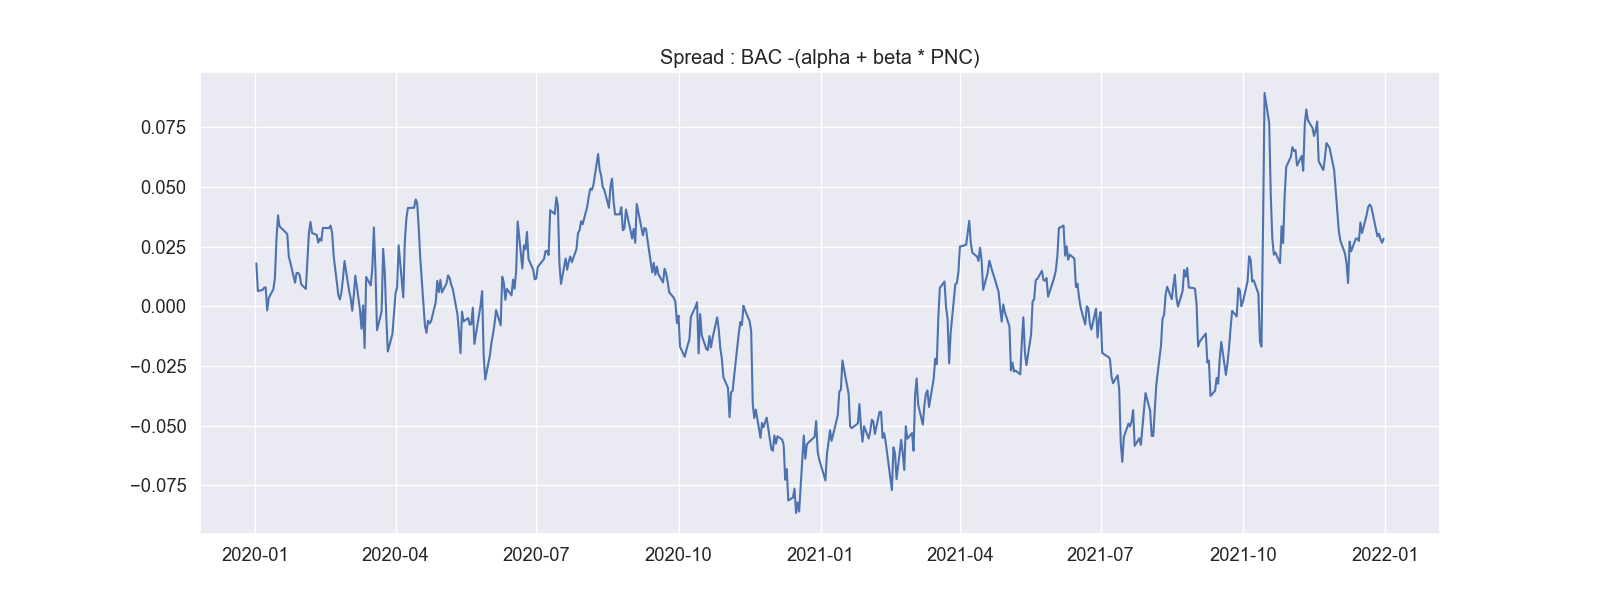
\includegraphics[width = 1\textwidth]{Figures/spread_bac.png}
	\caption{Residual/Spread of Regression of BAC on PNC}
	\label{fig:spread_bac}
\end{figure}
\FloatBarrier

$$\Delta e^{BAC}_t = \gamma e^{BAC}_{t-1} + \delta_1 \Delta e^{BAC}_{t-1} + \epsilon_t$$ 

We perform Augmented Dickey-Fuller Test on this Cointegrated BAC residual $e^{BAC}_t$ with lag 1 and conclude that it is stationary since p-value less than 0.05 threshold.

\begin{table}[!ht] 
\centering 
\resizebox{0.7\textwidth}{!} { 
\begin{tabular}{rrrr}
\toprule
test statistics & p-value & No of lagged values & No of observations \\
\midrule
-3.2165 & 0.0190 & 1 & 503 \\
\bottomrule
\end{tabular}} 
\caption {ADF test output on BAC Residual/Spread} 
\label {adf_bac_pnc} 
\end{table} 
\FloatBarrier

\end{enumerate}

\subsubsection{Engle-Granger Procedure Step 2}

We will now perform the 2nd step of Engle-Granger procedure which is to estimate the Equilibrium Correction Model(ECM), or error correction equations:

It is a static model that assumes stationary $y_t$ and $x_t$. A dynamic regression model uses several lagged values.

$$ y_t = \alpha y_{t-1} + \beta_0 + \beta_1 x_t + \beta_2 x_{t-1} + \epsilon_t$$

we would like to re-specify the model to equilibrium-correction form

$$ y_t - y_{t-1} =  \alpha y_{t-1} -y_{t-1} + \beta_0 + \beta_1 x_t + \beta_2 x_{t-1} + \epsilon_t$$

$$ \Delta y_t =  -(1-\alpha) y_{t-1}  + \beta_0 + \beta_1 \Delta x_t + (\beta_1 + \beta_2) x_{t-1} + \epsilon_t$$

$$ \Delta y_t=  \beta_1 \Delta x_t -(1-\alpha)\left[y_{t-1} - \frac{\beta_0}{1-\alpha} - \frac{\beta_1 + \beta_2}{1-\alpha} x_{t-1}\right] +  \epsilon_t  $$

$$ \Delta y_t =  \beta_1 \Delta x_t -(1-\alpha)\left[y_{t-1} - a_e -b_e x_{t-1}\right] +  \epsilon_t  $$

$$ \Delta y_t =  \beta_1 \Delta x_t -(1-\alpha)\left[y_{t-1} - a_e -b_e x_{t-1}\right] +  \epsilon_t  $$

$$ \Delta y_t =  \beta_1 \Delta x_t -(1-\alpha) e_{t-1} +  \epsilon_t  $$

where $y_t = a_e + b_e x_t$ is a static equilibrium model encapsulated within the relationship between non-stationary(integrated) $x_t$ and $y_t$.

\begin{enumerate}[A.]
\item
\textbf{Error correction equation ( PNC on BAC)}

$$\Delta P^{PNC}_t = \phi \Delta P^{BAC}_{t} - (1-\alpha) \text{Coint\_PNCBAC}_{t-1} + \epsilon_t $$

Here we check significance of  $ -(1- \alpha)$ term that ensures the correction the long run equilibrium.In error correction equation the  p-value is evaluated against t-distribution as is common for regression. We  reject  H0(that a regression coefficient is zero) because the corresponding  p-value is less than 5\%. Below table indicates regression coefficient is significantly different from zero.

We also observe that speed of correction $ -(1- \alpha) = -0.0294$ is very small, but is significant for cointegration to exist.

\textbf{Summary of Error correction equation ( PNC on BAC)} 
\begin{center}
\begin{tabular}{lclc}
\toprule
\textbf{Dep. Variable:}    &   $\Delta$ Price\_PNC    & \textbf{  R-squared (uncentered):}      &     0.806   \\
\textbf{Model:}            &       OLS        & \textbf{  Adj. R-squared (uncentered):} &     0.805   \\
\textbf{Method:}           &  Least Squares   & \textbf{  F-statistic:       }          &     1041.   \\
\textbf{Date:}             & Wed, 17 Jan 2024 & \textbf{  Prob (F-statistic):}          & 2.35e-179   \\
\textbf{Time:}             &     13:15:22     & \textbf{  Log-Likelihood:    }          &    1632.6   \\
\textbf{No. Observations:} &         504      & \textbf{  AIC:               }          &    -3261.   \\
\textbf{Df Residuals:}     &         502      & \textbf{  BIC:               }          &    -3253.   \\
\textbf{Df Model:}         &           2      & \textbf{                     }          &             \\
\textbf{Covariance Type:}  &    nonrobust     & \textbf{                     }          &             \\
\bottomrule
\end{tabular}
\begin{tabular}{lcccccc}
                           & \textbf{coef} & \textbf{std err} & \textbf{t} & \textbf{P$> |$t$|$} & \textbf{[0.025} & \textbf{0.975]}  \\
\midrule
\textbf{$\Delta$ Price\_BAC}       &       0.9057  &        0.020     &    45.535  &         0.000        &        0.867    &        0.945     \\
\textbf{Lag1\_Spread\_PNC} &      -0.0294  &        0.012     &    -2.471  &         0.014        &       -0.053    &       -0.006     \\
\bottomrule
\end{tabular}
\begin{tabular}{lclc}
\textbf{Omnibus:}       & 51.017 & \textbf{  Durbin-Watson:     } &    1.933  \\
\textbf{Prob(Omnibus):} &  0.000 & \textbf{  Jarque-Bera (JB):  } &  205.857  \\
\textbf{Skew:}          & -0.343 & \textbf{  Prob(JB):          } & 1.99e-45  \\
\textbf{Kurtosis:}      &  6.055 & \textbf{  Cond. No.          } &     1.70  \\
\bottomrule
\end{tabular}
%\caption{OLS Regression Results}
\end{center}

Notes: \newline
 [1] R² is computed without centering (uncentered) since the model does not contain a constant. \newline
 [2] Standard Errors assume that the covariance matrix of the errors is correctly specified.\\

\item
\textbf{Error correction equation ( BAC on PNC)}

$$\Delta P^{BAC}_t = \phi \Delta P^{PNC}_{t} - (1-\alpha) \text{Coint\_BACPNC}_{t-1} + \epsilon_t$$  

Here we check significance of  $-(1- \alpha) $ term that ensures the correction in long run equilibrium. In error correction equation the  p-value is evaluated against t-distribution as is common for regression. We reject  H0(that a regression coefficient is zero) because the corresponding  p-value is less than 5\%. Below table indicates regression coefficient is significantly different from zero.

We also observe that speed of correction $-(1- \alpha) = -0.0407$ is very small, but is significant for cointegration to exist.

\textbf{Summary of Error correction equation ( BAC on PNC)} 
\begin{center}
\begin{tabular}{lclc}
\toprule
\textbf{Dep. Variable:}    &   $\Delta$ Price\_BAC    & \textbf{  R-squared (uncentered):}      &     0.808   \\
\textbf{Model:}            &       OLS        & \textbf{  Adj. R-squared (uncentered):} &     0.807   \\
\textbf{Method:}           &  Least Squares   & \textbf{  F-statistic:       }          &     1054.   \\
\textbf{Date:}             & Wed, 17 Jan 2024 & \textbf{  Prob (F-statistic):}          & 1.97e-180   \\
\textbf{Time:}             &     16:28:04     & \textbf{  Log-Likelihood:    }          &    1637.1   \\
\textbf{No. Observations:} &         504      & \textbf{  AIC:               }          &    -3270.   \\
\textbf{Df Residuals:}     &         502      & \textbf{  BIC:               }          &    -3262.   \\
\textbf{Df Model:}         &           2      & \textbf{                     }          &             \\
\textbf{Covariance Type:}  &    nonrobust     & \textbf{                     }          &             \\
\bottomrule
\end{tabular}
\begin{tabular}{lcccccc}
                           & \textbf{coef} & \textbf{std err} & \textbf{t} & \textbf{P$> |$t$|$} & \textbf{[0.025} & \textbf{0.975]}  \\
\midrule
\textbf{$\Delta$Price\_PNC}       &       0.8887  &        0.020     &    45.484  &         0.000        &        0.850    &        0.927     \\
\textbf{Lag1\_Spread\_BAC} &      -0.0407  &        0.012     &    -3.339  &         0.001        &       -0.065    &       -0.017     \\
\bottomrule
\end{tabular}
\begin{tabular}{lclc}
\textbf{Omnibus:}       & 84.021 & \textbf{  Durbin-Watson:     } &    1.905  \\
\textbf{Prob(Omnibus):} &  0.000 & \textbf{  Jarque-Bera (JB):  } &  402.713  \\
\textbf{Skew:}          &  0.629 & \textbf{  Prob(JB):          } & 3.56e-88  \\
\textbf{Kurtosis:}      &  7.194 & \textbf{  Cond. No.          } &     1.61  \\
\bottomrule
\end{tabular}
%\caption{OLS Regression Results}
\end{center}

Notes: \newline
 [1] R² is computed without centering (uncentered) since the model does not contain a constant. \newline
 [2] Standard Errors assume that the covariance matrix of the errors is correctly specified.\\

\textbf{At the end, we select latter case - Error correction equation for BAC on PNC which has better t-statistics as compared to other case.}

\end{enumerate}

\pagebreak
\subsection{OU Process fitting}

The strategy trades the spread from the long/short portfolio(weights given  $\beta_{Coint}$).
For a mean-reversion arbitrage, we require the following items of information:

\begin{itemize}
\item Weights for a set of instruments $\beta_{Coint}$ to construct a spread.
\item Speed of mean-reversion in the spread $\theta$ to evaluate the feasibility of a trade.
\item Entry and exit levels together with the equilibrium level $\mu_e$, around which mean-reversion occurs. Fitting a spread to the Ornstein-Uhlenbeck process allows calculating the bounds as $$\sigma_{eq} \approx \frac{\sigma_{OU}}{\sqrt{2\theta}}$$
\end{itemize}

Appendix proof shows that the spread $e_t = \beta Y_t $ is an AR(1) process which makes it technically possible to perform fitting to the Ornstein-Uhlenbeck process and evaluate the speed of mean-reversion $\theta$ : the higher the $\theta$ the more stronger and less fractionated the cointegrated relationship is. That is possible to establish without conducting formal econometric tests for cointegration. Other fitted parameters, the equilibrium level $\mu_e$ and $\sigma_{eq}$ offer to calculate z-score given that $e_{t,\tau \to \infty} \thicksim N(\mu_e,\sigma^2_{eq}$).
OU fitting recipe uses the AR(1) model and is surprisingly simple as Eq \ref{eq:eq3}.
Parameters equilibrium level $\mu_e$, speed of mean reversion $\theta$ and diffusion $\sigma_{eq}$ are calculated are given as follows -

$$ \theta = - \frac{ln B}{\tau}, \mu_e = \frac{C}{1-B}, \sigma_{eq} = \sqrt{\frac{SSE/T}{1- e^{-2\theta\tau}}}$$
where where SSE is sum of squared residuals of AR(1) regression.\\

Comparison of the OU SDE solution to Equilibrium Correction mechanism Eq \ref{eq:eq7} gives an insightful representation, where all parameters fall in correct places with identifiable roles. In particular, the speed of adjustment towards the equilibrium is proportional to the autocorrelation of the OU process $\alpha \propto e^{-\theta\tau}$ , which is mean-reverting.

In order to give an indication of time required to generate the P\&L, the reversion speed can be presented as a global half-life: the time between the equilibrium situations of spread $e_t$ being at $\mu_e$.

$$\tilde{\tau} \propto \frac{ln 2}{\theta}$$

Mean-reversion begins with $\theta > 0$. The higher the theta the shorter half-life of reversion to the mean, and the better the quality of mean-reversion becomes.\\

\textbf{Summary of AR(1) model of BAC Spread(calculated from regression of BAC prices on PNC prices)}

\begin{center}
\begin{tabular}{lclc}
\toprule
\textbf{Dep. Variable:} &         BAC Spread        & \textbf{  No. Observations:  } &            505             \\
\textbf{Model:}         &         AutoReg(1)        & \textbf{  Log Likelihood     } &          1632.090          \\
\textbf{Method:}        &      Conditional MLE      & \textbf{  S.D. of innovations} &           0.009            \\
\textbf{Date:}          &      Wed, 17 Jan 2024     & \textbf{  AIC                } &         -3258.179          \\
\textbf{Time:}          &          18:17:20         & \textbf{  BIC                } &         -3245.512          \\
\textbf{Sample:}        &             1             & \textbf{  HQIC               } &         -3253.210          \\
\textbf{}               &            505            & \textbf{                     } &                            \\
\bottomrule
\end{tabular}
\begin{tabular}{lcccccc}
                       & \textbf{coef} & \textbf{std err} & \textbf{z} & \textbf{P$> |$z$|$} & \textbf{[0.025} & \textbf{0.975]}  \\
\midrule
\textbf{const}         &    1.839e-05  &        0.000     &     0.043  &         0.965        &       -0.001    &        0.001     \\
\textbf{BAC Spread.L1} &       0.9618  &        0.012     &    78.421  &         0.000        &        0.938    &        0.986     \\
\bottomrule
\end{tabular}
%\caption{AutoReg Model Results}
\end{center}

As we can see half-life is 17.7 days.
The speed of mean-reversion, in this case, is not very slow so we might expect reasonable number of trades when implementing the strategy that trades the spread by constructing a long/short portfolio.

\begin{table}[!ht] 
\centering 
\resizebox{0.7\textwidth}{!} { 
\begin{tabular}{rrrrr}
\toprule
B & C & Half Life & Equilibrium Level & Diffusion \\
\midrule
0.961767 & 0.000018 & 0.070559 & 0.000481 & 0.034662 \\
\bottomrule
\end{tabular}} 
\caption {OU Fitting Parameters on BAC Residual/Spread} 
\label {ou_fitting} 
\end{table} 
\FloatBarrier

\pagebreak
\section{Trading Strategy}

\subsection{Strategy formulation \& Assumptions}

\begin{enumerate}

\item At the end of each trading day, algorithm checks spread(residual) of BAC stock and decides trading 	signals based on $ \mu_{eq}, \sigma_{eq} and z $ values i.e. corresponding trading execution happens on subsequent day.
\item For long/short entry signals received at the end of day $T_1$, accumulation of returns will start from subsequent day ($T_1$ +1). Similarly, for long/short exit signal received at the end of day $T_2$, accumulation of returns will end on same day ($T_2$).
\item  Based on the optimization of P\&L, we get optimal Z value and approach is as follows:
\begin{enumerate}
\item To take long position (1 unit long position of BAC stock and beta units short position of PNC stock) when
spread $e_t$ crosses upper bound $\mu_{eq} + Z_{optimnal} \sigma_{eq} $ from below, and there is no position.
When spread $e_t$ reverts to value $\mu_{eq}$ then exit the position.
\item Similarly, to take short position (1 unit short position of BAC stock and beta units long position of PNC stock) when spread $e_t$ crosses lower bound $\mu_{eq} - Z_{optimnal} \sigma_{eq} $ from above, and there is no position. When spread $e_t$ reverts to value $\mu_{eq}$ then exit the position.
\end{enumerate}
\item This is an example of \textbf{Buy \& Hold} strategy, means we take either long or short position on spread based on entry signal and hold it until we get exit signal for the same. \textbf{There is no rule for accumulation of position}
\item we calculate gross returns and net returns (based on user-defined fee percent parameter - this includes transaction cost, brokerage fee etc) i.e. whenever we take new position or exit existing position, fee percent is deducted from gross returns to arrive at net returns.

\end{enumerate}

\subsection{Optimization of Z  value based on Cumulative P\&L }

Based on Strategy cumulative P\&L, we get optimal Z value as 0.8 which has number of trades as 25 including both entry and exit sides.

\begin{table}[!ht] 
\centering 
\resizebox{0.4\textwidth}{!} { 
\begin{tabular}{rrr}
\toprule
Z Values & No Trades & Net Strategy PL \\
\midrule
0.4000 & 41 & 1.5331 \\
0.5000 & 37 & 1.3693 \\
0.6000 & 29 & 1.3599 \\
0.7000 & 25 & 1.4677 \\
0.8000 & 25 & 1.6416 \\
0.9000 & 21 & 1.4404 \\
1.0000 & 17 & 1.3572 \\
1.1000 & 11 & 1.2205 \\
1.2000 & 11 & 1.2090 \\
1.3000 & 9 & 1.1771 \\
1.4000 & 7 & 1.1621 \\
1.5000 & 7 & 1.1904 \\
1.6000 & 7 & 1.1792 \\
\bottomrule
\end{tabular}} 
\caption {No of Trades, Strategy PL for Z values} 
\label {z_values} 
\end{table} 
\FloatBarrier

\begin{figure}[ht]
	\centering
	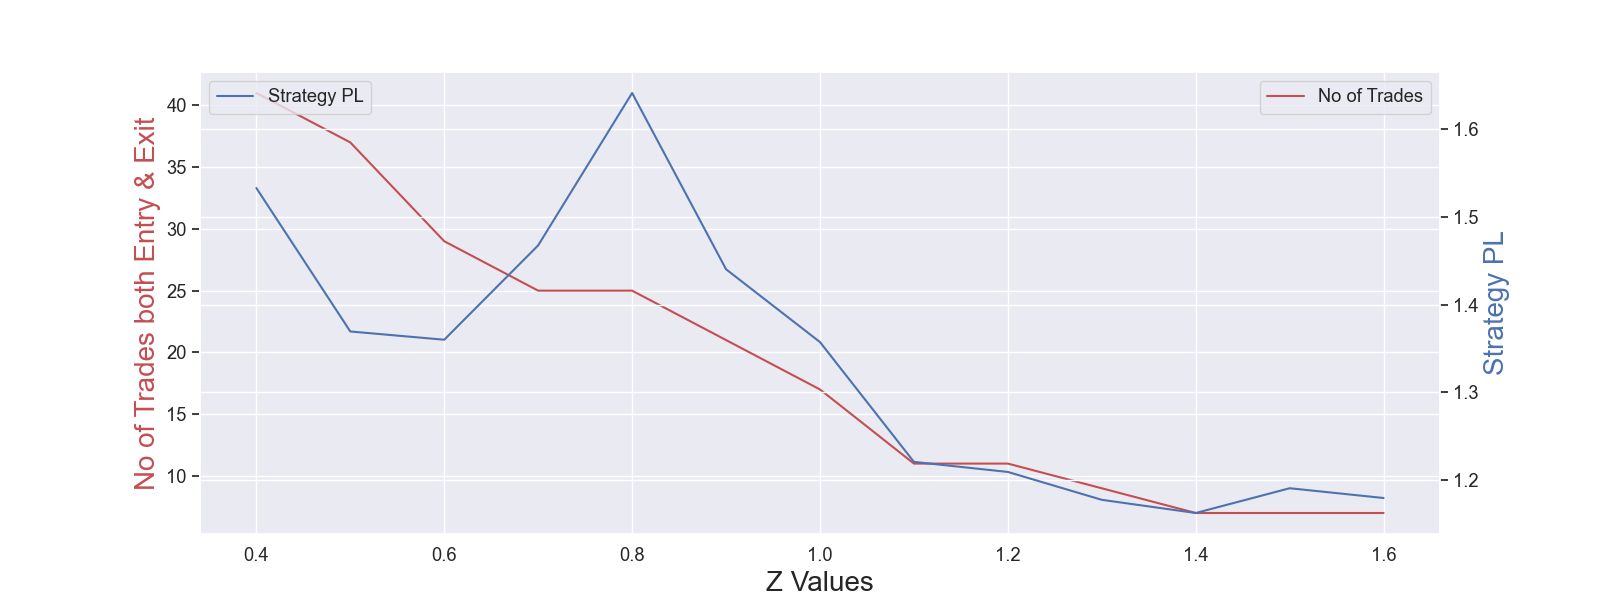
\includegraphics[width = 1\textwidth]{Figures/z_values.png}
	\caption{No Trades, Strategy P\&L for Z Values}
	\label{fig:z_values}
\end{figure}
\FloatBarrier

Fig \ref{fig:spread_bound} shows upper bound as 0.0282 and lower bound as -0.0272 with equilibrium level as 0.0005 for trading signals.

\begin{figure}[ht]
	\centering
	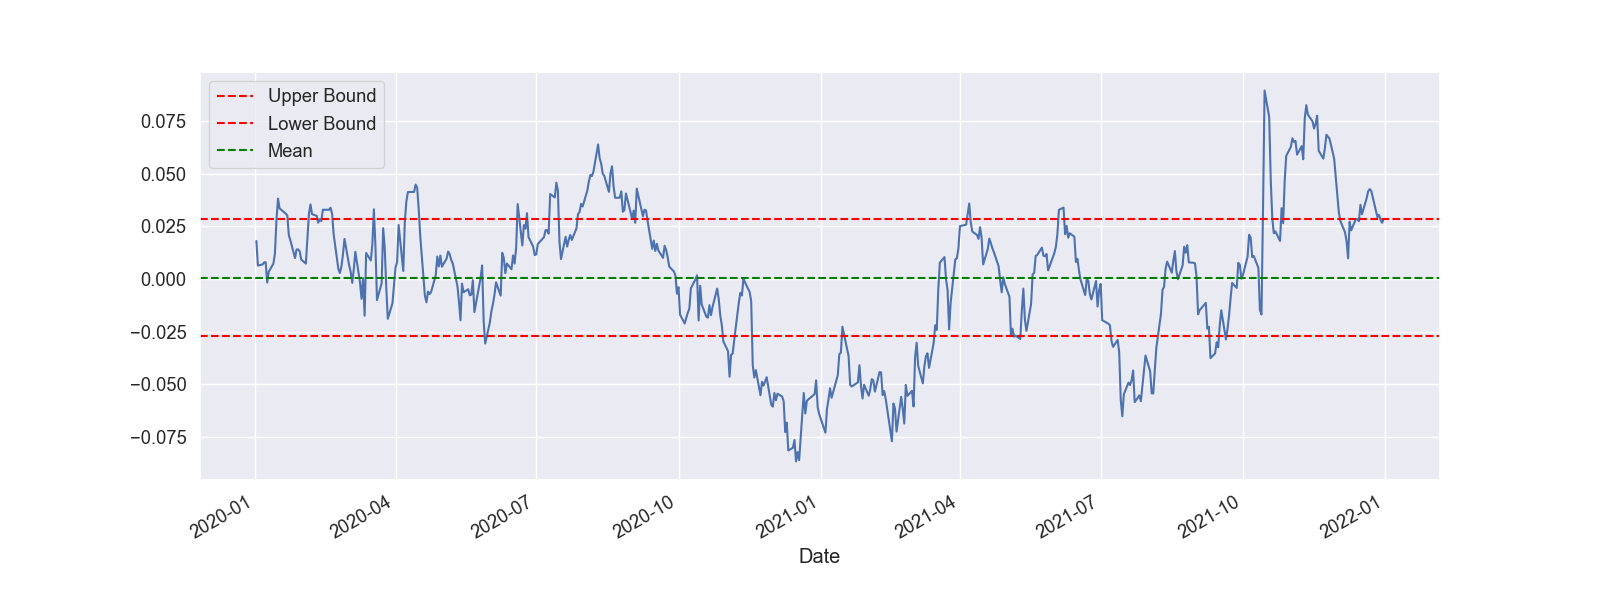
\includegraphics[width = 1\textwidth]{Figures/spread_bound.png}
	\caption{Trading Signals : Upper/Lower Bounds \& Equilibrium Level}
	\label{fig:spread_bound}
\end{figure}
\FloatBarrier

\subsection{Strategy P\&L and comparison with Benchmark P\&L}

\textbf{Strategy P\&L Results \& Limitations}

\begin{enumerate}

\item Pairs trading strategy can help to get good returns regardless of the conditions of the market. Hence,  the pair trading strategy can earn good returns it leverages on the opportunity when one asset is undervalued/overvalued wrt other asset in pair.
\item Here, we observe that strategy P\&L is delivering $\sim$  86\% gross return and $\sim$ 64\% net return (fee percent : 0.5\%) in 2 years period  and it is exceeding market return $\sim$ 46\% in the same period. Hence we conclude that strategy is working well and can be suitable for real-life implementation.
\item We also observe that, strategy is performing better than benchmark index particularly in falling market conditions.
\item We did not include concept of stop-loss in trading strategy design. However, due to risk management policies/governance, sometimes it is mandatory to keep stop-loss limits for trading positions to avoid heavy losses i.e. spread takes much more time to revert to equilibrium level.
\item Cointegrated relationship supposed to persist and $\beta_{Coint}$ should stay the same. Practitioners advice cited in several sources suggest of using one/two year of historic data and trade the estimates for a six-month period. Based on same rationale, we selected 2 years of training set and six months of test set for our analysis.

\end{enumerate}

\begin{figure}[ht]
	\centering
	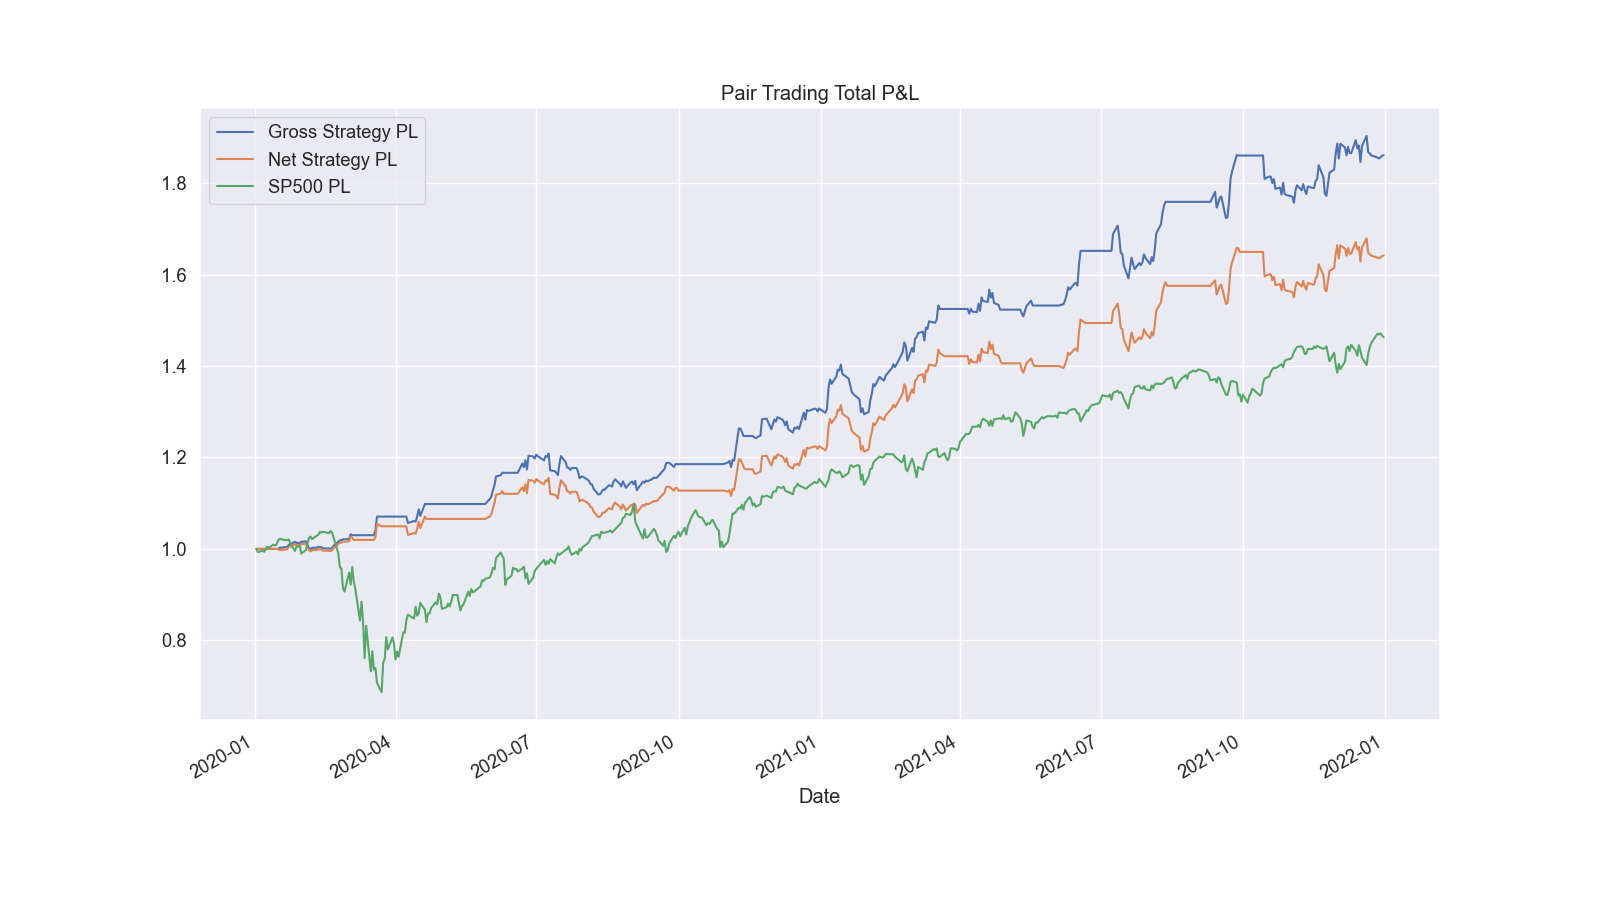
\includegraphics[width = 1\textwidth]{Figures/strategy_pnl.png}
	\caption{Strategy P\&L and comparison with S\&P 500 P\&L  }
	\label{fig:strategy_pnl}
\end{figure}
\FloatBarrier

\pagebreak
\section{Backtesting of Trading Strategy}

Now that we have constructed our spread appropriately and have an idea of how we will go about making trades, it is time to conduct some out of sample testing. Our whole model is based on the premise that these securities are cointegrated, but we built it on information from a certain time period. If we actually want to implement this model, we need to conduct an out of sample test to confirm that the principles of our model are still valid going forward. Historical results do not guarantee future results so this is a sanity check to see if the work we have done holds strong.

\subsection{Machine learning-inspired Backtesting}

For ML based backtesting of trading starategy, we use test dataset which contains stock prices data from Jan-2022 to Jun-2022.

\begin{figure}[htbp!]
	\centering
	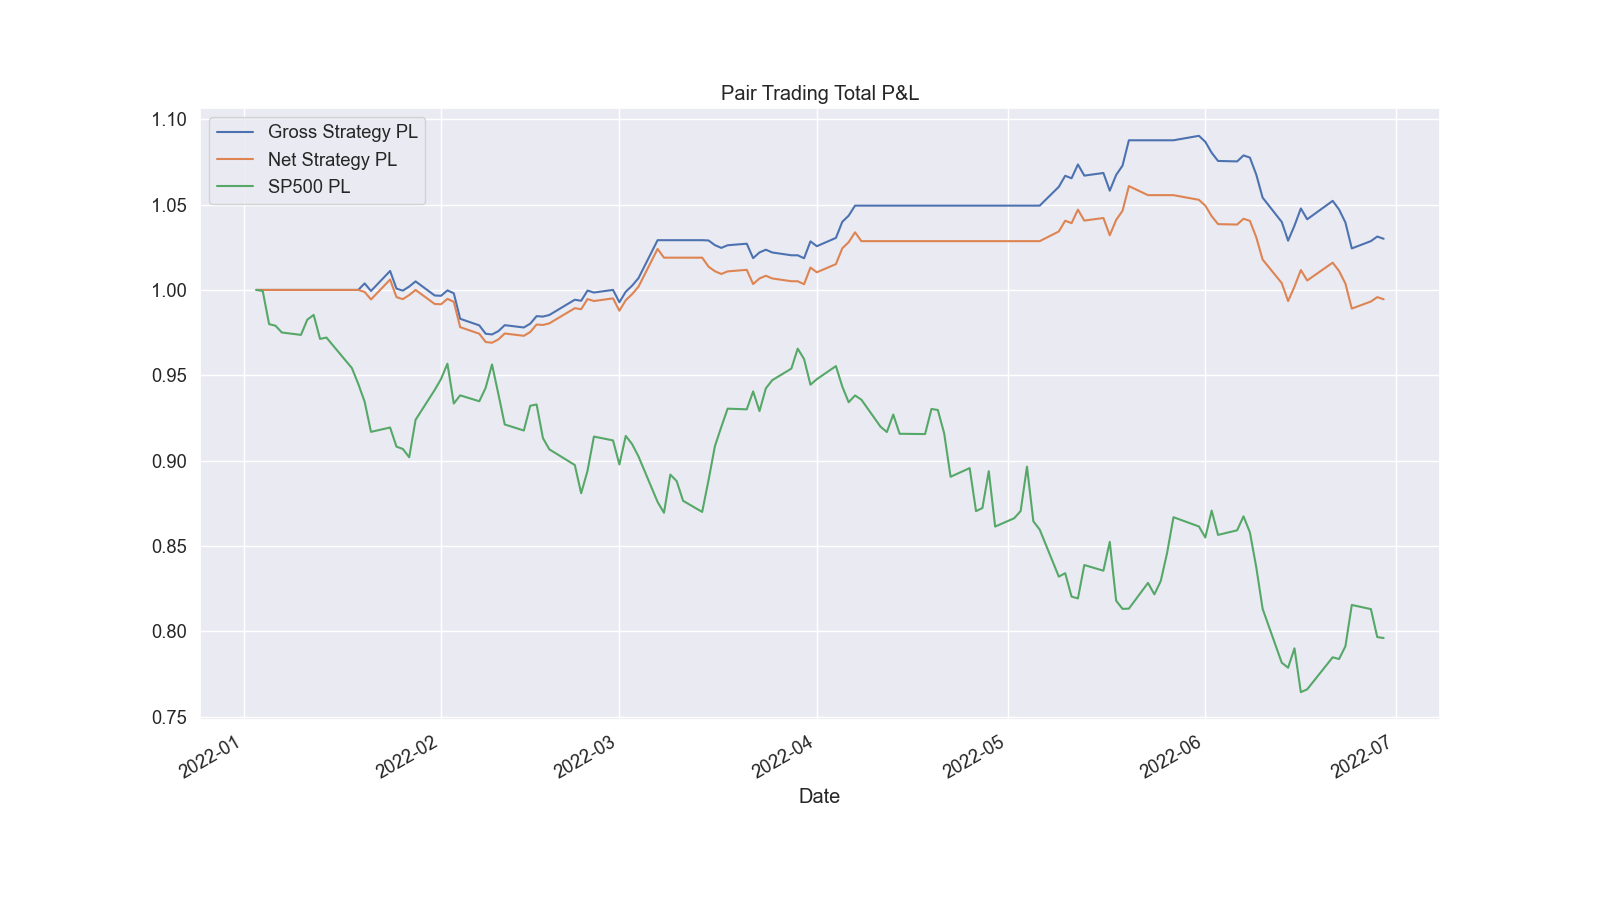
\includegraphics[width = 1\textwidth]{Figures/backtest_pnl.png}
	\caption{Backtesting P\&L and comparison with S\&P 500 P\&L  }
	\label{fig:strategy_pnl}
\end{figure}
\FloatBarrier

\textbf{Backtesting P\&L Results \& Areas of Improvement}

\begin{enumerate}

\item  Here, we observe that backteting P\&L is delivering $\sim$ 3\% gross return and flat net return (fee percent : 0.5\%) in six-months period, however it is exceeding negative market returns in the same period. Hence we conclude that out of sample testing of trading strategy is still delivering excellent results.
\item For the pairs trading strategy cointegration test, we only used a handful of stocks. Naturally (and in practice) it would be more effective to use clusters within an industry.
\item \textbf{Dealing with overfitting} - Anything related to data analysis and training models has much to do with the problem of overfitting. There are many different ways to deal with overfitting like validation, such as Kalman filters, and other statistical methods.
\item Cointegrated relationship supposed to persist and $\beta_{Coint}$ should stay the same. However, it is not always the case and sometimes,cointegrated relationships require regular re-estimation- Kalman filter or particle filter adaptive estimation can be useful here.

\end{enumerate}

\subsection{Portfolio Risk-Return Analytics}
\begin{table}[!ht]
\resizebox {0.4\textwidth}{!} 
{
\begin{tabular}{lc}
\toprule
\textbf{Start date}         &   2022-01-03     \\
\textbf{End date}         &     2022-06-29 \\
\textbf{Total months}        &   5  \\
\textbf{}        &   \textbf{Backtest}  \\
\textbf{Annual return}        &   -1.1\%  \\
\textbf{Cumulative returns}        &   -0.5\%  \\
\textbf{Annual volatility}        &   8.7\%  \\
\textbf{Sharpe ratio}        &   -0.09  \\
\textbf{Calmar ratio}        &   -0.17 \\
\textbf{Stability}        &   0.38  \\
\textbf{Max drawdown}        &   -6.8\%  \\
\textbf{Omega ratio}        &   0.98  \\
\textbf{Sortino ratio}        &   -0.12  \\
\textbf{Skew}        &   0.24  \\
\textbf{Kurtosis	}        &   2.30  \\
\textbf{Tail ratio}        &   0.94  \\
\textbf{Daily value at risk} & 	-1.1\% \\
\textbf{Alpha}        &   -0.02  \\
\textbf{Beta}        &   -0.04  \\
\end{tabular}
}

\resizebox {1.1\textwidth}{!} 
{

\begin{tabular}{cccccc}
\toprule
\textbf{Worst drawdown periods}       &  \textbf{Net drawdown in \%} & \textbf{Peak date} &   \textbf{Valley date} & \textbf{Recovery date} &  \textbf{Duration} \\
0     &  6.76 & 2022-05-20 &    2022-06-24 & NaT & NaN  \\
1     &  3.68 & 2022-01-24 &   2022-02-09 &    2022-03-07 & 31 \\
2     & 2.02 & 2022-03-07 &   2022-03-30 &  2022-04-05  &  22  \\
3     &  1.43 & 2022-05-12 &    2022-05-17 &  2022-05-20	 &  7 \\
4     &  0.56 & 2022-01-19 &     2022-01-21	  &  2022-01-24   & 4   \\
\bottomrule
\end{tabular}
}
\end{table}
\FloatBarrier

\begin{figure}[htbp!]
	\centering
	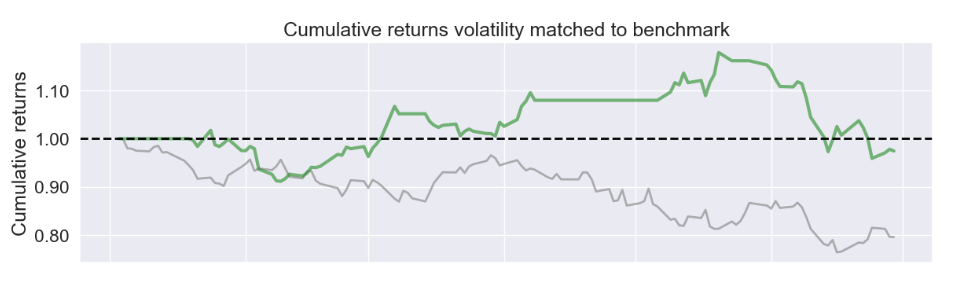
\includegraphics[width = 1\textwidth]{Figures/Cumulative returns volatility matched to benchmark.png}
	\label{fig:Cumulative returns volatility matched to benchmark}
\end{figure}
\FloatBarrier

\begin{figure}[htbp!]
	\centering
	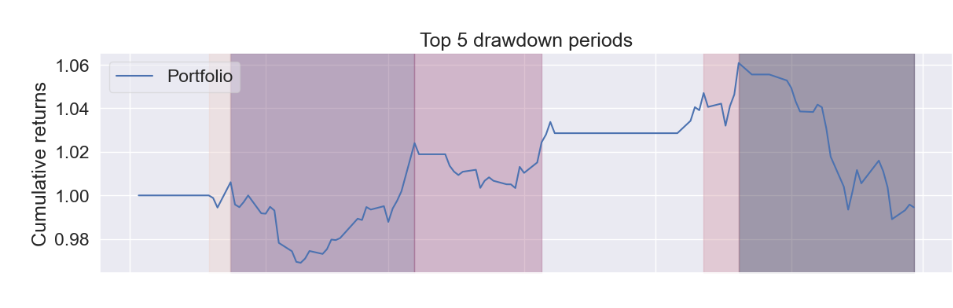
\includegraphics[width = 1\textwidth]{Figures/Top 5 drawdown periods.png}
	\label{fig:Top 5 drawdown periods}
\end{figure}
\FloatBarrier

\begin{figure}[htbp!]
	\centering
	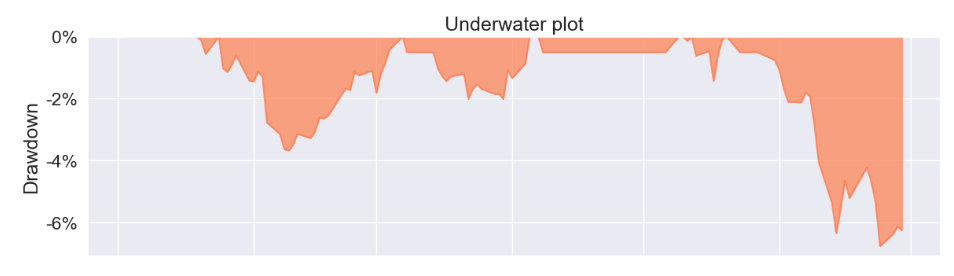
\includegraphics[width = 1\textwidth]{Figures/Underwater plot.png}
	\label{fig:Underwater plot}
\end{figure}
\FloatBarrier

\begin{figure}[htbp!]
	\centering
	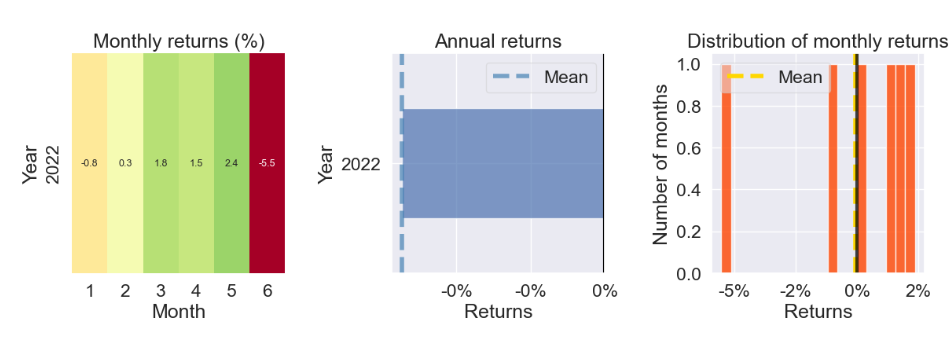
\includegraphics[width = 1\textwidth]{Figures/pf_returns_1.png}
	\label{fig:pf_returns_1}
\end{figure}
\FloatBarrier

\begin{figure}[htbp!]
	\centering
	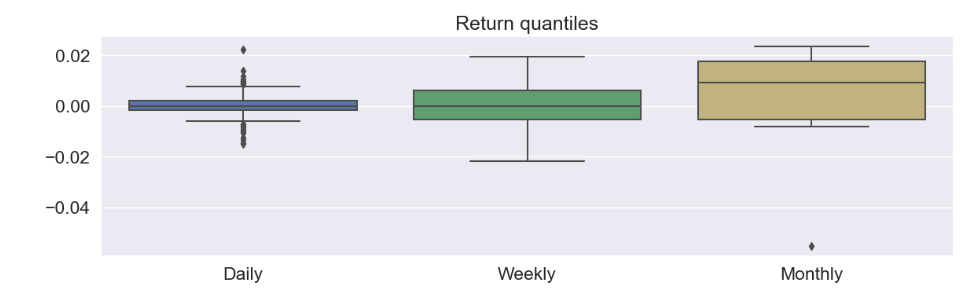
\includegraphics[width = 1\textwidth]{Figures/pf_returns_2.png}
	\label{fig:pf_returns_2}
\end{figure}
\FloatBarrier

\subsection{Rolling Sharpe}

While the traditional Sharpe ratio gives a single snapshot, the rolling Sharpe ratio provides a moving picture, recalculating the ratio over a fixed period as new data comes in. This rolling calculation offers a more immediate and ongoing analysis of the risk-adjusted performance, allowing investors to spot trends, volatility, and the impact of market events on investment returns.

The standard Sharpe ratio for strategy returns is given by the following formula:

$$S = \frac{\mathbb{E}(R_s - R_f)}{\sqrt{Var(R_s - R_f)}}$$
Where $R_{s}$ refers to the strategy return and  $R_{f}$ refers to risk free return i.e. We have taken US Treasury bill rate as risk free rate in calculation.

In order to calculate an k-days rolling Sharpe ratio it is necessary to make two modifications to this formula. The first is to reduce the set of returns to the last trailing number of k-days trading periods (e.g. for daily data this means take the last k-days close-to-close returns). The second is to multiply the value by the square root of the number of k-days periods. 

$$S_t = \sqrt{k}\frac{\mathbb{E}(R_{s,t-k} - R_{f,t-k})}{\sqrt{Var(R_{s,t-k} - R_{f,t-k})}}$$

Where $R_{s,t-k}$ refers to the previous truncated strategy returns.\\

\textbf{from the below plot, we observe 1-month Rolling Sharpe Ratio is very volatile which is not desirable i.e. one of the reasons is less number of trades available due to short trading window of 6 months}

\begin{figure}[htbp!]
	\centering
	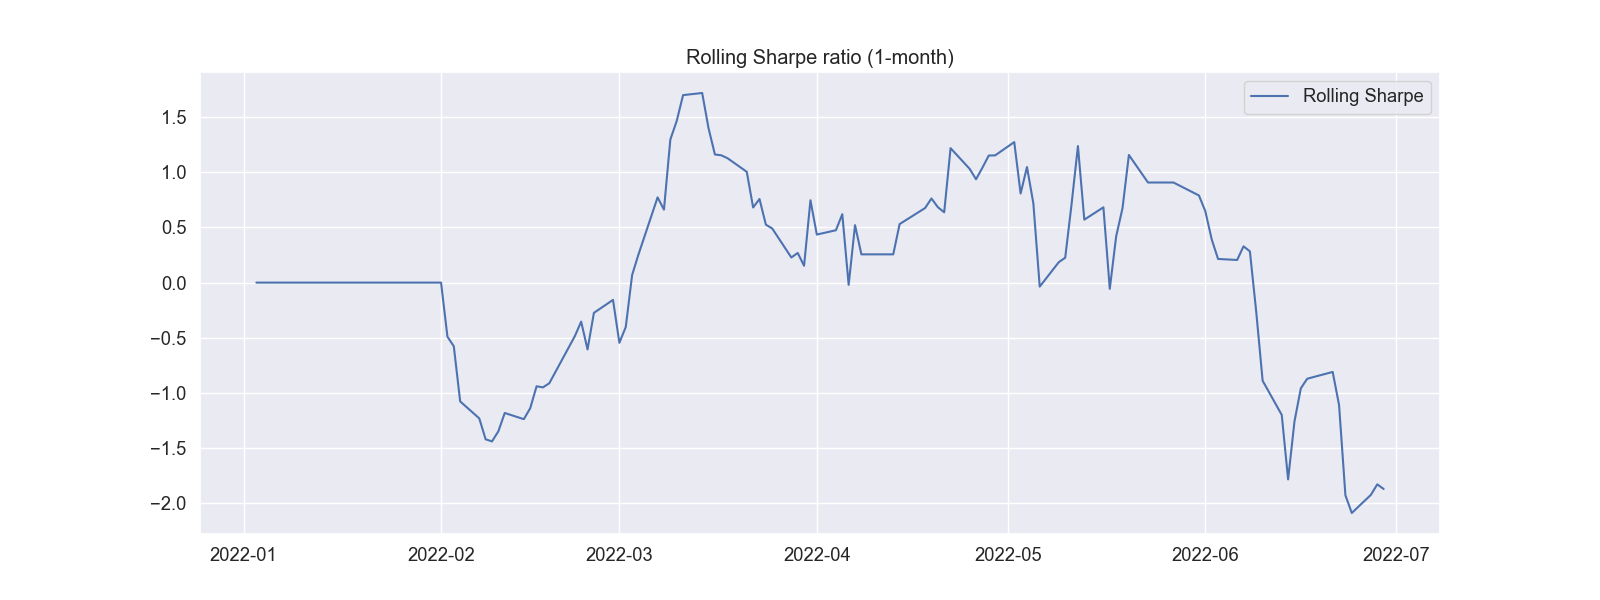
\includegraphics[width = 1\textwidth]{Figures/roling_sharpe.png}
	\label{fig:roling_sharpe}
\end{figure}
\FloatBarrier

\subsection{Rolling Beta}

\begin{itemize}
\item $\beta > 1$ : If strategy beta above 1, then it means that its return, on average, moves more than 1 to 1 with the return of the index.
\item $\beta < 1$: If strategy beta below 1, then it means that its return, on average, moves less than 1 to 1 with the return of the index.
\item $\beta = 0$: It means that the strategy tends to have an opposite direction to the market.
\end{itemize}

\begin{figure}[htbp!]
	\centering
	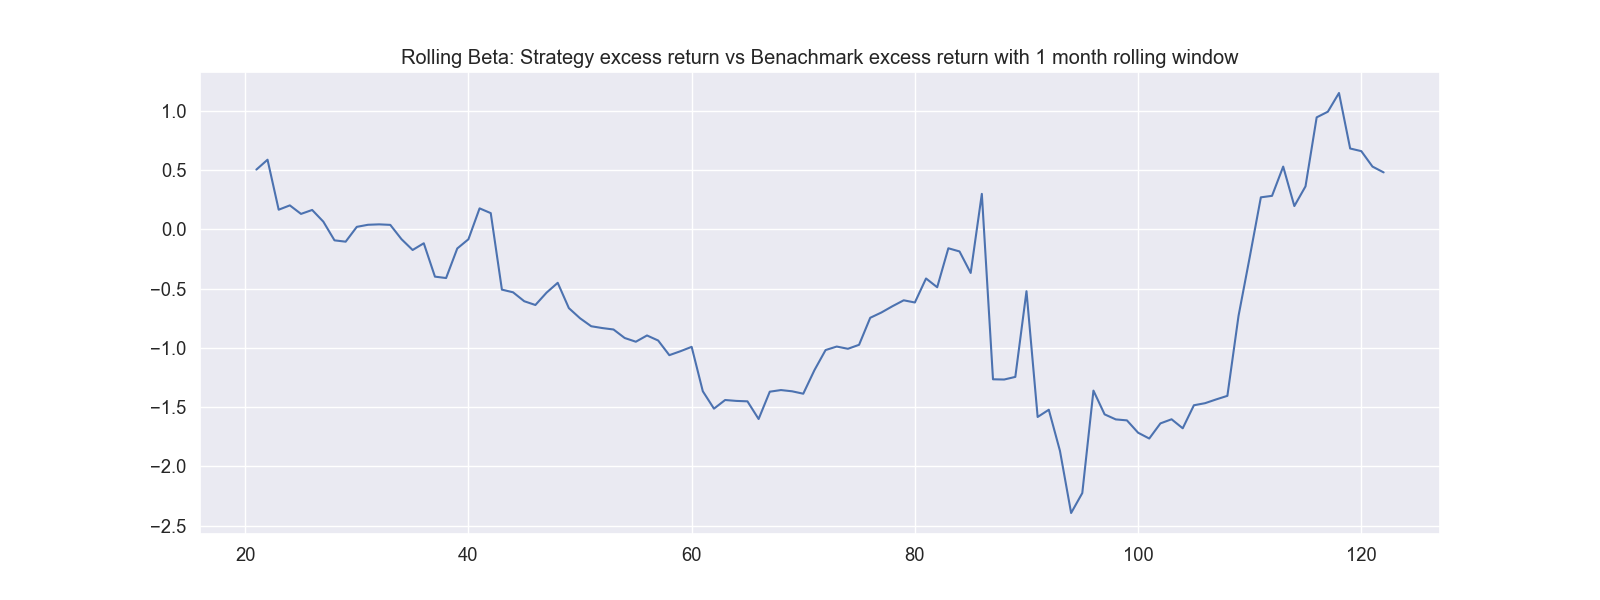
\includegraphics[width = 1\textwidth]{Figures/roling_beta.png}
	\label{fig:roling_beta}
\end{figure}
\FloatBarrier

Here, we observe that 1-month Rolling beta(strategy excess return vs S\&P 500 index excess  return) is quite volatile i.e. ranging from negative to positive values. Since rolling beta is not very stable and hence this might not be as relevant to start arbitrage and market-making activities.

\pagebreak

\section{References}

\begin{enumerate}[ {[}1{]} ]
\item \textit{Pairs Trading with Cryptocurrencies} : by Sergey Malchevskiy Available at\\
\url{https://towardsdatascience.com/pairs-trading-with-cryptocurrencies-e79b4a00b015}

\item \textit{Cointegration and Pairs Trading} : by Letian Wang Available at\\
\url{https://letianzj.github.io/cointegration-pairs-trading.html}

\item \textit{Vector Autoregressive models VAR(p) models} : The Pennsylvania State University Lectures\\
 Available at \url{https://online.stat.psu.edu/stat510/lesson/11/11.2}

\item \textit{A Guide to Conducting Cointegration Tests} : by Eric Available at\\
\url{https://www.aptech.com/blog/a-guide-to-conducting-cointegration-tests/}
 
\item \textit{Learning and Trusting Cointegration in Statistical Arbitrage} : by Richard V. Diamond \\
Available at \url{https://papers.ssrn.com/sol3/papers.cfm?abstract_id=2220092}

\item \textit{An Introduction to Cointegration for Pairs Trading} : by Yefeng Wang \\
Available at \url{https://hudsonthames.org/an-introduction-to-cointegration/}

\item \textit{CQF Lecture on Cointegration for Trading} : by Richard V. Diamond 

\end{enumerate}

\pagebreak

\section{Appendix}

\subsection{Ornstein-Uhlenbeck Process(Quality of Mean-Reversion)}

We use the process in order to model the residual of cointegrating relationship (vector error term) $e_t = \beta_{coint} Y_t$, given its statistical properties of being stationary AR(1) process with frequent mean reversion around $\mu_e$ .Its SDE gives a continuous representation of an autoregressive process with the mean-reversion $\theta$ and 
and diffusion $\sigma_{OU} $.

\begin{equation} \label{eq:eq1} de_t = -\theta(e_t - \mu_e) dt + \sigma_{OU} dX_t \end{equation} 

the regression-like solution in continuous time t + $\tau$ 

\begin{equation} \label{eq:eq2} e_{t+\tau} = (1 -e^{-\theta \tau}) \mu_e + e^{-\theta \tau} e_t + \epsilon_{t,\tau}\end{equation} 

OU SDE solution offers two terms: reversive and autoregressive

Autoregressive equivalent for a small time period $\tau$ is

\begin{equation} \label{eq:eq3} e_{t+\tau} = C + B e_t + \epsilon_{t,\tau} \end{equation}

Once AR(1) is estimated, we can solve for equilibrium level $\mu_e$  and speed of mean reversion $\theta$

$$ \theta = - \frac{ln B}{\tau}, \mu_e = \frac{C}{1-B}$$ 

The following comparison shows that the Ornstein-Uhlenbeck process fit matches the features of equilibrium-correction term, which is commonly present in econometric cointegration models.
\begin{equation} \label{eq:eq4} e_{t+\tau} = (1 -e^{-\theta \tau}) \mu_e + e^{-\Theta \tau} e_t \end{equation} 

\begin{equation} \label{eq:eq5} e_{t+\tau} - e_t + e_t -e^{-\theta \tau} e_t = (1 -e^{-\theta \tau}) \mu_e \end{equation} 

\begin{equation} \label{eq:eq6} \Delta e_{t,\tau} + (1-e^{-\theta \tau})e_t = (1 -e^{-\theta \tau}) \mu_e \end{equation}

\begin{equation} \label{eq:eq7} \Delta e_{t,\tau} = - (1 -e^{-\theta \tau})(e_t -\mu_e) \end{equation}

now compare this bivariate ECM equation

\begin{equation} \label{eq:eq8} \Delta e_{t,\tau} = -(1-\alpha) (y_{1,t} - \beta y_{2,t} - \mu_e) \end{equation}

Introduction of the equilibrium level $\mu_e$ means that we model $\Delta e_{t,\tau}$. Otherwise that level should be moved outside of the cointegrating relationship and seen as a constant growth rate.

\end{document}
